\documentclass[12pt,a4paper]{article}
% packages
\usepackage[margin=2cm]{geometry}
\usepackage{graphicx}
\usepackage{algorithmic}
\usepackage{algorithm}

\parskip = 12pt
\parindent = 0pt
\linespread{1.5}

% xCJK
\usepackage[boldfont]{xCJK}
\setCJKmainfont{AR PL New Kai}
\begin{document}
\begin{CJK*}{UTF8}{song}

\CJKspace
\begin{titlepage}

\begin{center}

\begin{Large}
教育部主辦\\[1cm]
九十七學年度大學校院\\[1cm]
積體電路電腦輔助設計軟體製作競賽\\[1cm]
競 賽 報 告
\end{Large}

\vfill

\begin{large}
報名編號:   \\
組  別:定題組
\end{large}

\vfill

\begin{Large}
Failure Candidate Identification for Silicon Debug
\end{Large}

\vfill

\begin{large}
中華民國九十七年 12 月 28 日
\end{large}

\end{center}

\end{titlepage}



\section{Abstract}

  在第一個 silicon prototype 被大量製造以前,首要的事情就是確認製造%
的過程和系統的整合,而下圖表示在 silicon prototype 被大量製造以前,%
silicon 所要作的測試。

\begin{center}
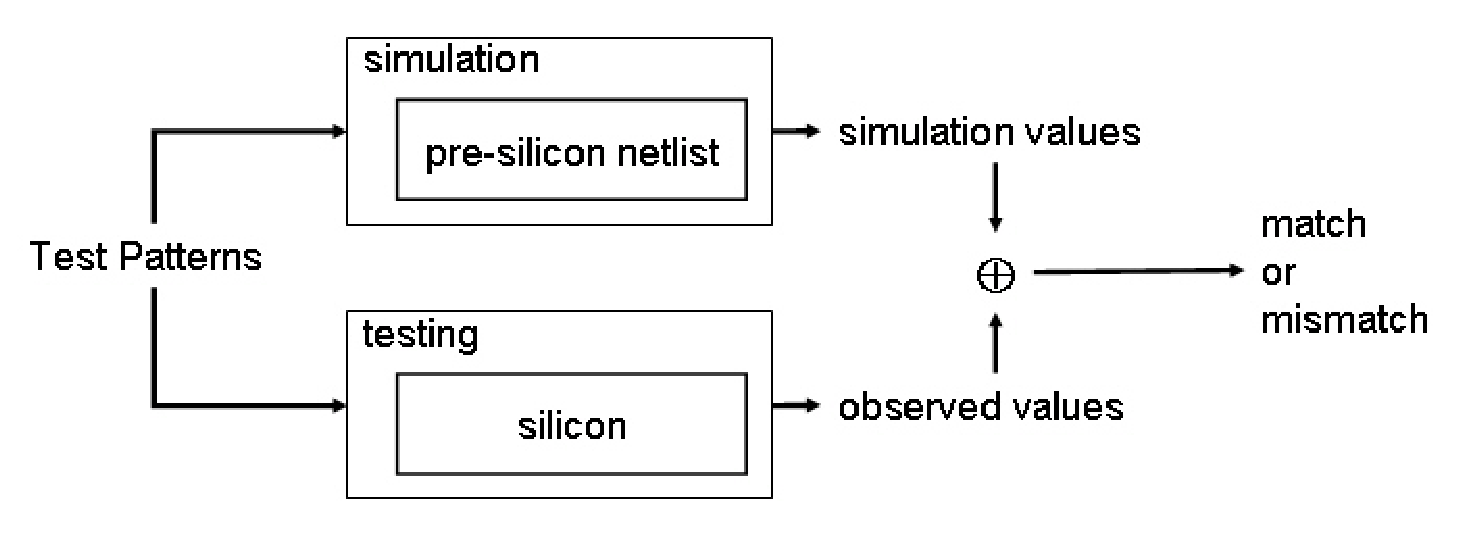
\includegraphics[scale=0.6]{imgs/01.eps}
\end{center}

  當我們拿到 test pattern 後,我們會做兩種測試,分別為 simulation %
和 testing,如果兩種測試出來的結果相同,則就是 match,不同的話則是%
 mismatch,而我們所做的程式,則是在得到 mismatch 後,對於 silicon %
prototype 做 debug,找出裡面有可能的 defective signal。

\section{Introduction}

\subsection{Problem Description}

  給予以下三個 input 檔案:

\begin{enumerate}
\item verilog 的 pre-silicon flatten gate-level netlist。
\item silicon 作 simulation 所有 signal 的 dump value。
\item silicon 做 testing 最後所得到的 output value。
\end{enumerate}

我們要做 debug,找出所有可能的 defective signal。

  為了能找出 mismatch behavior,我們使用 what-if 這個方法,%
藉由改變目前的 value,我們可以快速的找出問題所在,在這裡,我們只討論%
一次改變一個 signal。以下圖的 n2 為例,我們將 n2 的 1 改變為 0,則 O1、%
n4 和 O2 的 value 皆會改變,如果改變後的 output 與 testing 觀察所得到%
的 value 一樣的話,那麼 n2 可能就是一個 defective signal。

\begin{center}
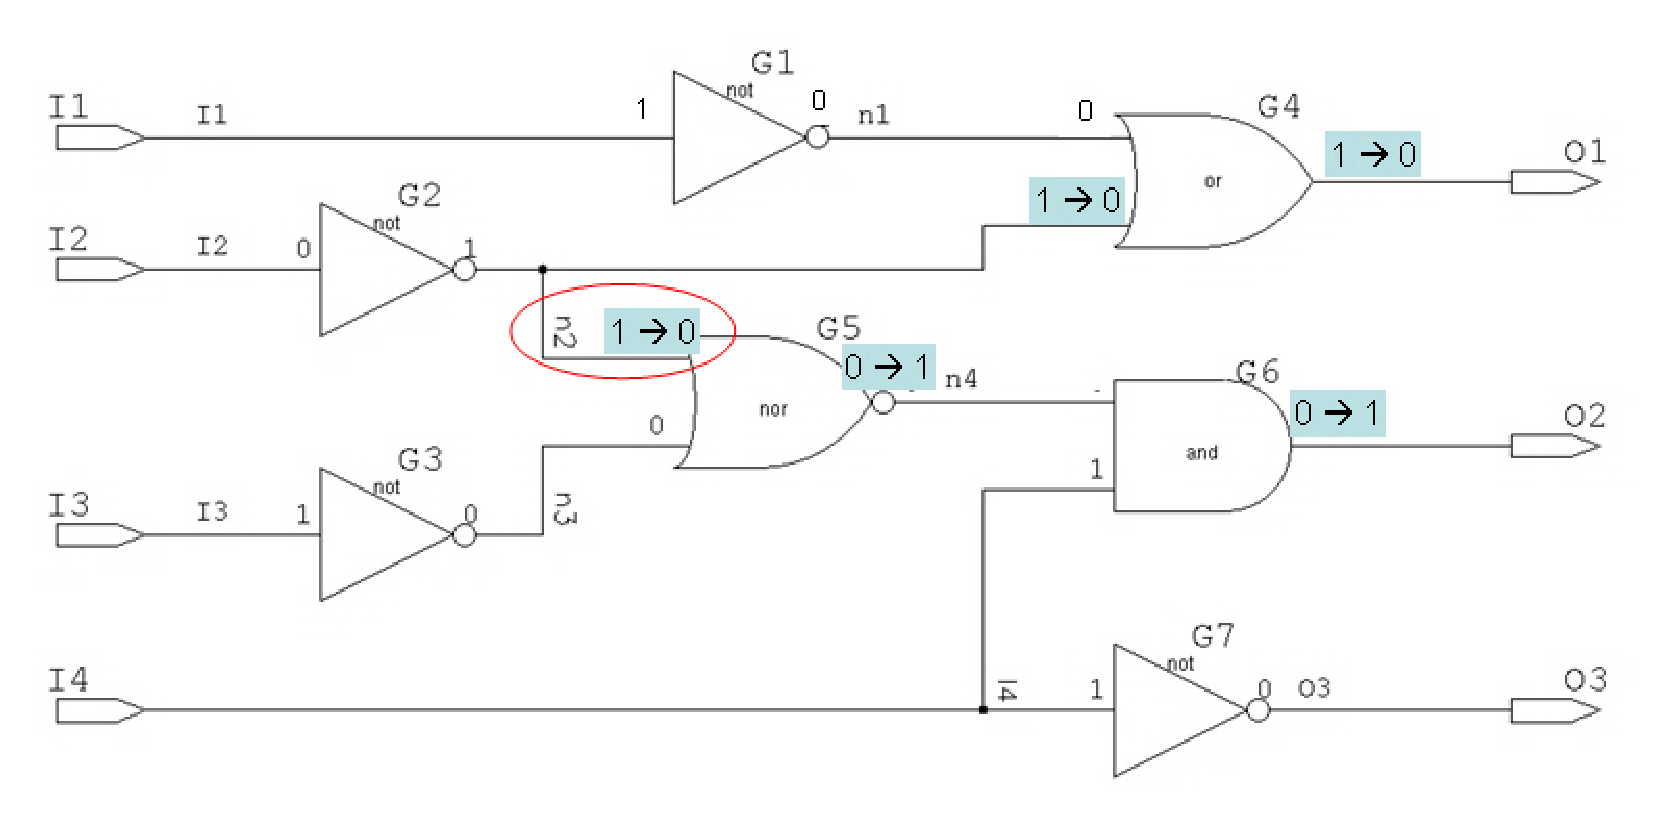
\includegraphics[scale=0.6]{imgs/02.eps}
\end{center}

  因此,我們需要一個程式,能夠將所有可能的 defective signal 給%
找出來,並且利用一些演算法,找出有可能是 defective signal 的 signal,%
再對這些 signal 做 what-if 分析,如此一來,可以減少很多不必要%
的 what-if 分析,以達到 debug 最大的效率。

\subsection{Functions and Features}

  本軟體依照上述的需求,完成所應該要做的分析,並且利用%
兩個演算法,減少不必要的 what-if 分析,在最短的時間內%
把有作 what-if 的 signal 和最後有可能的 defective signal 給列出來。%

\subsection{Contributions and Results}

  為了減少不必要的 what-if analysis,我們依照題目的提示%
設計了兩個演算法,分別為 Static approach 和 Dynamic approach,%
利用這兩種演算法,我們便可以提升程式的效率。

\section{Algorithms}

  以下是主要的演算法,詳細的的 pseudo code 在最後一頁。

{\linespread{1}

\begin{algorithm}
\caption{$analysis(output\_set, observed\_set)$}
\begin{algorithmic}[1]
\STATE $diff\_set \leftarrow output\_set \setminus observed\_set$
\STATE $candidates \leftarrow \{\}$
\STATE $finals \leftarrow \{\}$
\STATE $breadth\_first\_traversal(diff\_set, static\_analysis(candidates))$
\FOR{each $item$ in $candidates$}
    \STATE perform what-if analysis for $item$
    \IF{the evaluated signals is equal to observed values}
        \STATE insert $item$ into $finals$
    \ELSE
        \STATE $breadth\_first\_traversal(item, dynamic\_analysis(candidates))$
    \ENDIF
\ENDFOR
\RETURN $(candidates, finals)$
\end{algorithmic}
\end{algorithm}

}

\subsection{$analysis$ line $1$}

  因為要找出 defective signal,對於沒有改變的 output 不予理會,%
所以將 simulation dump 中 output 部份與 observed value 取補集,%
得到部份的 output node,以減少分析的數量。%

\begin{center}
\begin{minipage}{0.3\textwidth}
\center
simulation dump
\hrule
\begin{verbatim}
O1 = 1
O2 = 0
O3 = 0
\end{verbatim}
\end{minipage}
\begin{minipage}{0.3\textwidth}
\center
observed value
\hrule
\begin{verbatim}
O1 = 0
O2 = 1
O3 = 0
\end{verbatim}
\end{minipage}
\end{center}

  上面為範例,我們將兩者取補集,進而得到 O1、O2 兩 node。

\subsection{$analysis$ line $4$}

  從 output 往 input 的方向執行 breadth-first traversal,%
在 traverse 過程中對經過的元件進行 static analysis。%
以下是 static analysis 的說明。

\begin{center}
\begin{tabular}{|c|c|c|c|c|c|c|}
\hline
p & q & and & nand & or & nor & xor\\
\hline
0 & 0 & 0   & 1    & 0  & 1   & 0\\
\hline
1 & 0 & 0   & 1    & 1  & 0   & 1\\
\hline
0 & 1 & 0   & 1    & 1  & 0   & 1\\
\hline
1 & 1 & 1   & 0    & 1  & 0   & 0\\
\hline
\end{tabular}
\end{center}

  由上表可知,當 and gate 的 output 為 $0$,只有 input 為 $0$ 的部份會影響結果,%
又從題目可知一次只有一個 signal 會發生改變,當兩 input 為 $0$ ,%
即使其中一個改變,output 依然不受影響。

  因為是從 output 往 input 進行 traverse,當我們知道某個 input 不會造成影響,%
便可以停止對該元件繼續往 input 方向 traverse,即使後面的元件發生改變,%
對目前的 output 也不會有影響。

  因此,當元件為 and gate,我們將其 input 為 $0$ 的元件放入 $candidates$ 裡面,%
並且只對此元件繼續往下進行 travere,其他 input 則不予理會。

  至於 nand、or、nor 也是以相同的原理進行篩選。

\begin{center}
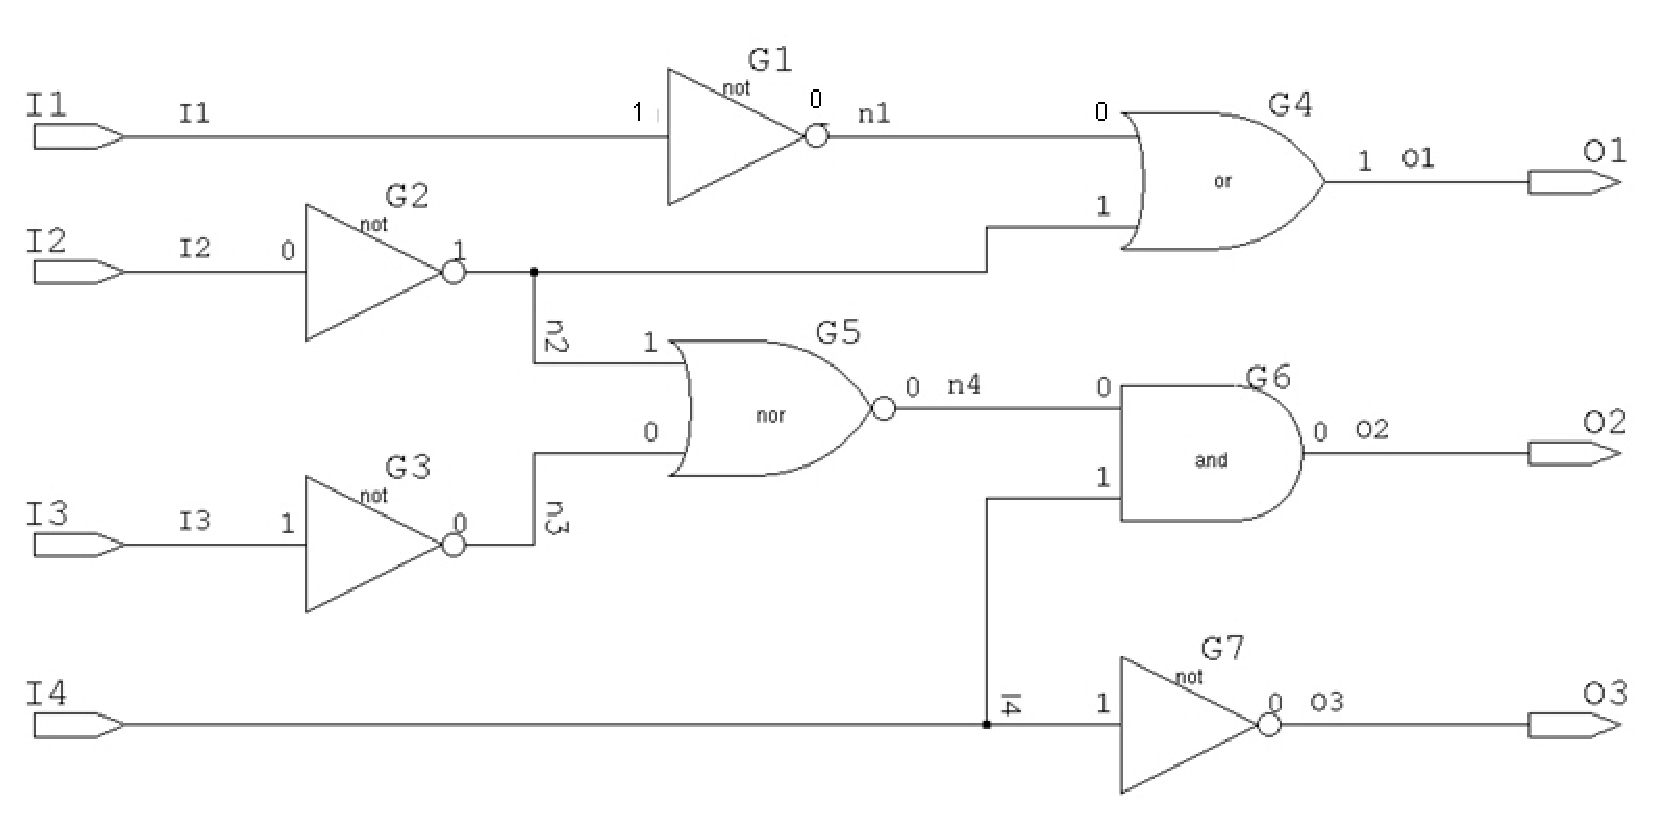
\includegraphics[scale=0.6]{imgs/04.eps}
\end{center}

  以上圖為例,從 output 開始進行 breadth-first traversal,%
依序走訪 O1、O2,並將其 G4、G6 放到 $queue$。當走到 G4 時發現其 output value 為 $1$,%
並且 n2 為 $1$、n1 為 $0$,我們可以確定 n1 不會造成影響,%
所以僅把 n2 放入 $queue$ 以及 $candidates$,然後繼續走訪 G6 分析其 input node。

\subsection{$analysis$ line $5..12$}

  對 $candidates$ 的元件依序進行 what-if analysis,判斷是否為 defective signal,%
如果執行之後的結果與 observed value 一樣,便將此元件放入 $finals$;%
如果不同,就對該元件從 output 往 input 的方向執行 breadth-first traversal,%
在 traverse 過程中對經過的元件進行 dynamic analysis。

  我們所作的 dynamic analysis 是,如果已知元件不是 defective signal,%
便從 $candidates$ 刪除僅與此元件連接的 input node。%
因為只有與目前的元件連線,所以可以確定刪除之後不會對尚未作 what-if 的元件造成影響。%
刪除後並往 input node 的方向 traverse,繼續進行 dynamic analysis。

\begin{center}
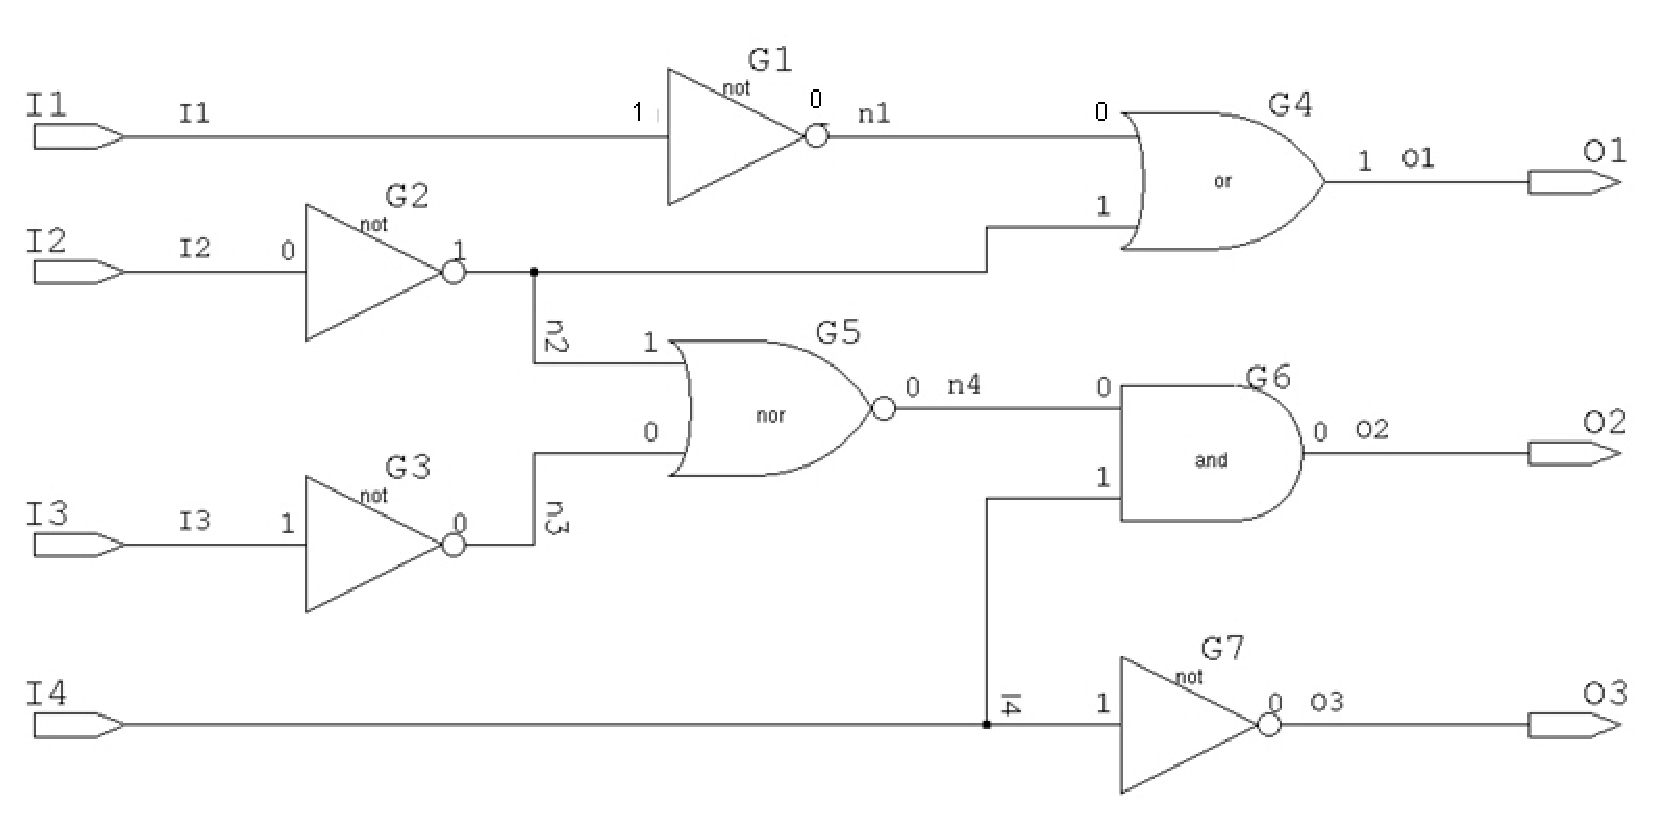
\includegraphics[scale=0.6]{imgs/04.eps}
\end{center}

  以上圖為例,假設對 n1 進行 what-if analysis,發現不是 defective signal,%
便從 n1 開始執行 breadth-first traversal。走到 G1 時發現 I1 存在於 $candidates$ %
並只有與 G1 連接,我們便把它從 $candidates$ 刪除,並把它放入 $queue$ 繼續往下走訪。

\section{Implementation}

\subsection{Data Structure}

  我們將 design.v 讀進來,以 map 對應每個元件的 id 至實際的 node。%
元件的 structure 如下

\begin{verbatim}
struct item {
    std::string id;
    int value;
    bool visited;
    item_list input;
    item_list output;
};
\end{verbatim}

$value$ 是 simulation dump value,$input$ 是元件的 input node,%
$output$ 是元件的 output node。

  至於 sim.dump 與 obs.dump 則是以 map 對應元件 id 至各個數值。

\begin{verbatim}
map["I1"] == 1;
map["n1"] == 0;
map["O1"] == 0;
\end{verbatim}

\subsection{Flow}

\begin{center}
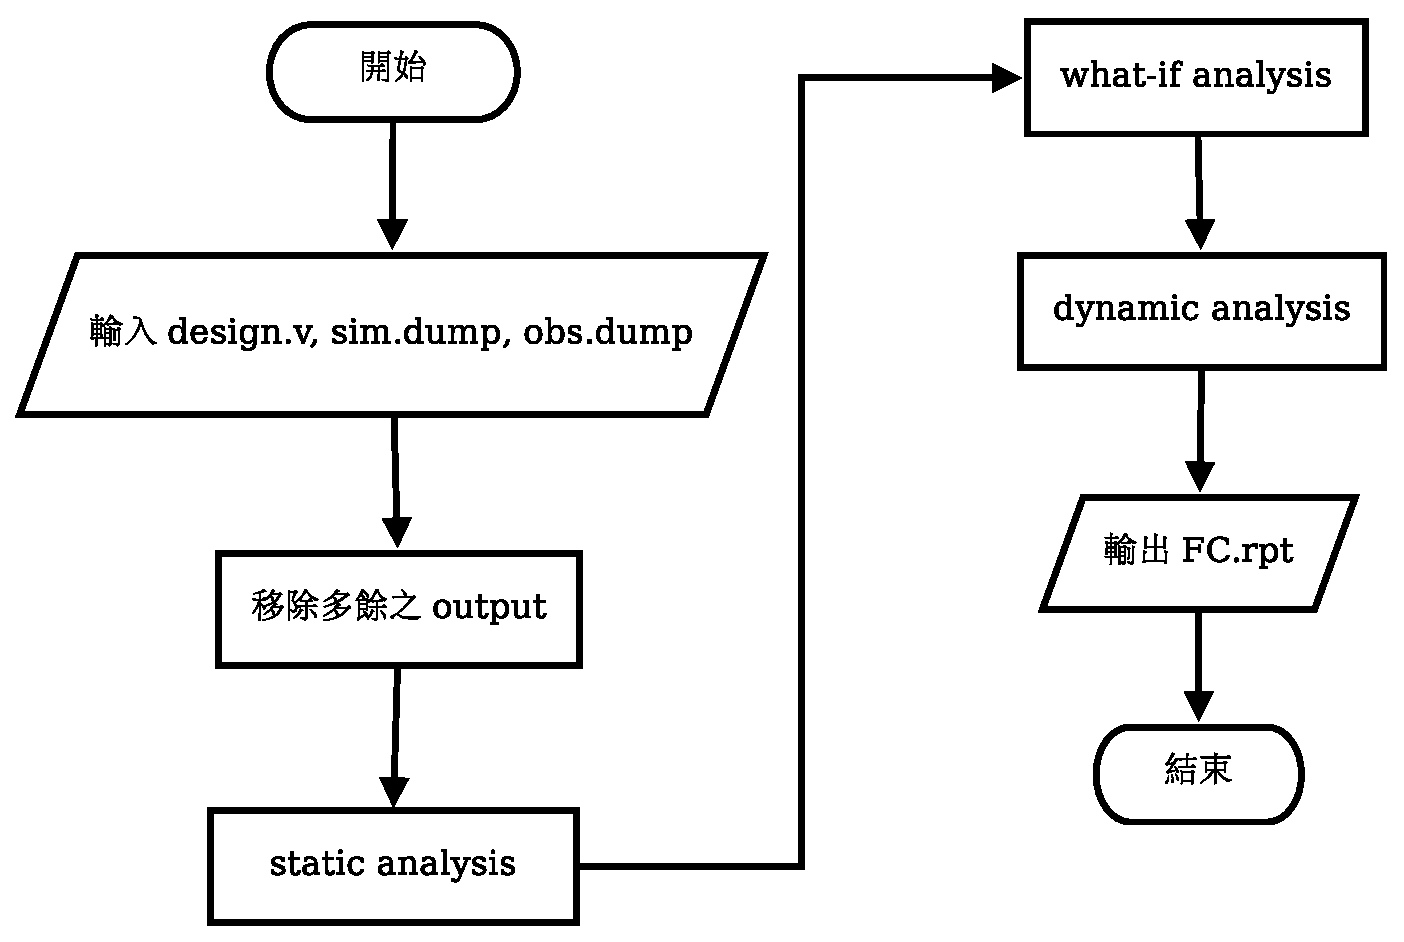
\includegraphics[scale=0.6]{imgs/03.eps}
\end{center}

\section{Experimental Results}

\subsection{Platform and Programming Language}

\begin{itemize}
\item 作業系統:Debian GNU/Linux x86
\item 處理器 :Intel Core2 Duo 1.80GHz
\item 記憶體 :2048 MB (DDR2 667)
\item 程式語言:C++
\item 編譯器 :g++ 4.3.2
\item library :boost 1.37
\end{itemize}

\subsection{Test Output}

  經由主辦單位提供之兩個資料作測試,以下是測試結果

Case 1
\hrule
\begin{verbatim}
Number of performing the ‘what-if’ analysis: 3
W1
I1
I3

Number of final candidates: 3
W1
I1
I3
\end{verbatim}

Case 2
\hrule
\begin{verbatim}
Number of performing the ‘what-if’ analysis: 7
W8
W2
O1
W6
I2
W5
W3

Number of final candidates: 6
W8
W2
O1
W6
I2
W3
\end{verbatim}

\subsection{CPU Time and Memory Usage}

\begin{tabular}{|l|l|l|}
  \hline
               & Case 1 & Case 2\\
  \hline
  components   & 17     & 31\\
  \hline
  time    & 0 sec  & 0 sec\\
  \hline
  memory  & 0 KB   & 0 KB\\
  \hline
\end{tabular}

  為取得程式資源的使用量,我們使用 GNU time 進行量測,但因測試資料數量不大,%
測量出來的 CPU time 與 memory usage 分別為 $0$ sec 及 $0$ KB

\section{Appendix}

\subsection{User Manual}

\begin{enumerate}
\item  解壓縮:tar zxvf eda-project.tar.gz
\item 進入目錄:cd eda-project
\item   編譯:make
\item   執行:./identifyFC -netlist design.v\\
           -sim\_dump sim.dump\\
           -obs\_dump obs.dump\\
           -out FC.rpt
\end{enumerate}

\subsection{Pseudo code}

{\linespread{1}

\begin{algorithm}
\caption{$static\_analysis(candidates, item)$}
\begin{algorithmic}[1]
\STATE $in$ $\leftarrow$ input items of $item$
\IF{($item$ is and gate $\land$ output signal of $item$ is $0$) $\lor$\\
($item$ is nand gate $\land$ output signal of $item$ is $1$)}
    \STATE $x$ $\leftarrow$ items of $in$ which signal is $0$
    \IF{amount of $x$ is equal to $1$}
        \STATE insert $x$ into $candidates$
        \RETURN $x$
    \ENDIF
\ELSIF{($item$ is or gate $\land$ output signal of $item$ is $1$) $\lor$\\
($item$ is nor gate $\land$ output signal of $item$ is $0$)}
    \STATE $x$ $\leftarrow$ items of $in$ which signal is $1$
    \IF{amount of $x$ is equal to $1$}
        \STATE insert $x$ into $candidates$
        \RETURN $x$
    \ENDIF
\ELSIF{$item$ is wire $\lor$ $item$ is input $\lor$ $item$ is output}
    \RETURN $in$
\ELSE
    \STATE insert $in$ into $candidates$
    \RETURN $in$
\ENDIF
\RETURN \{\}
\end{algorithmic}
\end{algorithm}

\begin{algorithm}
\caption{$dynamic\_analysis(candidates, item)$}
\begin{algorithmic}[1]
\STATE $in$ $\leftarrow$ input items of $item$
\STATE $next = \{\}$
\IF{$item$ is wire $\lor$ $item$ is input $\lor$ $item$ is output}
    \RETURN $in$
\ENDIF
\FOR{each $out$ in output items of $in$}
    \IF{$out$ is not in $candidates \setminus \{item\}$}
        \STATE remove $in$ from $candidates$
        \STATE insert $in$ into $next$
    \ENDIF
\ENDFOR
\RETURN $next$
\end{algorithmic}
\end{algorithm}

\begin{algorithm}
\caption{$breadth\_first\_traversal(root, next\_children)$}
\begin{algorithmic}[1]
\STATE $queue \leftarrow \{root\}$
\WHILE{$queue$ is not empty}
    \STATE $node \leftarrow pop(queue)$
    \STATE $children \leftarrow next\_children(node)$
    \STATE insert $child$ into $queue$
\ENDWHILE
\end{algorithmic}
\end{algorithm}

}

\end{CJK*}
\end{document}
